\begin{appendix}
\section*{Extra Scatter Plots}
\begin{figure}[H]
    \centering
    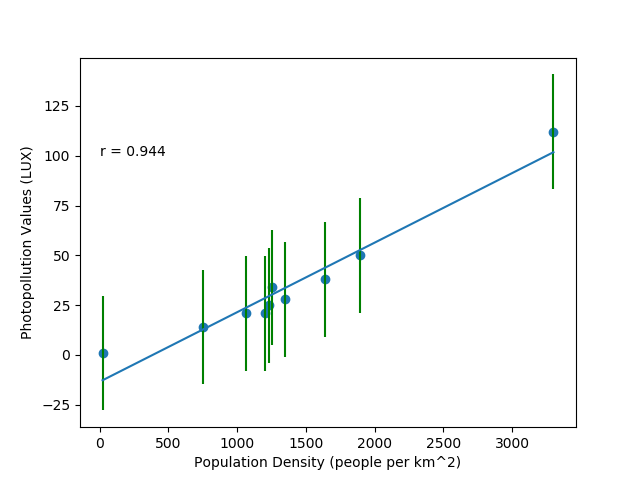
\includegraphics[width=.8\linewidth]{meanluxfirst}
    \caption{Mean Photopollution Values (First Site)}
    \label{meanluxfirst}
\end{figure}
\begin{figure}[H]
    \centering
    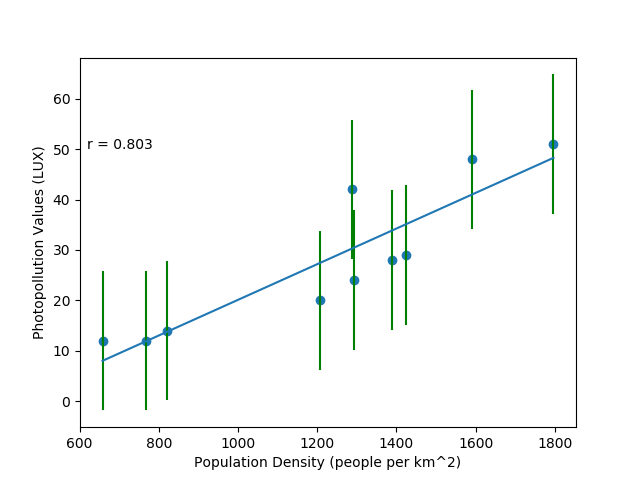
\includegraphics[width=.8\linewidth]{meanluxsecond}
    \caption{Mean Photopollution Values (Second Site)}
    \label{meanluxsecond}
\end{figure}

\newpage

\section*{Extra Table}
\begin{tabularx}{\textwidth}{|X|l|}
  \hline
  \textbf{The Name of the Site Visited} & \textbf{Mean Photopollution Value} \\ [15pt]
\hline
Blackwater Bridge (Dark Site) & 1 LUX \\ [15pt]
\hline
Tipperary Town & 21 LUX \\ [15pt]
\hline
Cahir & 28 LUX \\ [15pt]
\hline
Clonmel & 38 LUX \\ [15pt]
\hline
Ballymacarbry & 14 LUX \\ [15pt]
\hline
Lismore & 34 LUX \\ [15pt]
\hline
Tallow & 21 LUX \\ [15pt]
\hline
Watergrasshill & 50 LUX \\ [15pt]
\hline
Cork City & 112 LUX \\ [15pt]
\hline
Macroom & 25 LUX \\ [15pt]
\hline
Tarbert & 12 LUX \\ [15pt]
\hline
Kilrush & 14 LUX \\ [15pt]
\hline
Ennis & 42 LUX \\ [15pt]
\hline
Shannon & 28 LUX \\ [15pt]
\hline
Limerick City & 47 LUX \\ [15pt]
\hline
Adare & 24 LUX \\ [15pt]
\hline
Newcastle West & 29 LUX \\ [15pt]
\hline
Tralee & 20 LUX \\ [15pt]
\hline
Killarney & 51 LUX \\ [15pt]
\hline
Kenmare & 12 LUX \\ [15pt]
\hline
\end{tabularx}

\newpage

\section*{Python Programs}
\subsection*{Solver Program}
\lstinputlisting[language=Python, breaklines=true]{Python_Code_for_LaTex/Solver.py}

\hfill

\subsubsection*{Main Program}
\lstinputlisting[language=Python, breaklines=true]{Python_Code_for_LaTex/Program.py}

\section*{Email Correspondences with Prof. Brian Espey}

\author{Conor Casey \\ email \href{mailto:16ccasey@student.kenmarecs.com}{16ccasey@student.kenmarecs.com} 
   \and Prof. Brian Espey \\ email \href{mailto:someone@somewhere.com}{someone@somewhere.com} 
}

\textbf{From: Conor Casey, To: Prof. Brian Espey}

I am doing a project called “Is It Possible to Create a Mathematical Model to Predict Photopollution Based on Population Density in Munster” for the BTYSTE 2019.
I am contacting you to enquire if you would be willing to answer some questions on light pollution. The answers to these questions would be included in my Project Book. 


\textbf{From: Prof. Brian Espey, To: Conor Casey}

Hi Conor,

Sure- send the questions on. I presume that you've done some research and come across the Walker model for light pollution? see, e.g. adsbit.harvard.edu/cgi-b...e=.pdf

Best regards,

Brian.



\textbf{From: Conor Casey, To: Prof. Brian Espey}

Professor Espey,
Thank you for responding to my email. It is greatly appreciated.
I had not previously seen this particular paper before, however, I am familiar with the Walker model.
I have a number of questions to ask you:

1)  What equipment/apparatus did you use to carry out your observations for Light Pollution in the Irish Context.

2)  You make reference several times in your research to the comparison between Northern Ireland and the Republic in terms of light pollution? Did you make any measurements in Northern Ireland and if so how many and at what sites?

3) Do you think the unit LUX is an appropriate unit of measurement for photopollution?

4) Could population density be a lurking variable in the Walker Model? As in, due to the fact that population density decreases with an  increased distance from the city centre (CBD), could population density actually be responsible as opposed to distance and population size. I have attached a link discussing the relationship between population and distance from the central business district in relation to population size:
adsbit.harvard.edu/cgi-b...e=.pdf

5) Why in the Walker Model, $\frac{mag}{sec^{2}}$ is the unit of measurement used?

I also wanted to enquire if the Trinity Physics Department would be willing to take Transition Year students for work experience, if so who should I contact.


\textbf{From: Professor Brian Espey, To: Conor Casey}

Hello Conor,

See the text below each question for answers.

Hope this helps- let me know if you have more questions.

Brian.

\textbf{Answers:}

I have used a combination of the Sky Quality Meter equipment

(www.unihedron.com) in both the hand-held SQM, SQM-L models and also the datalogging equipment. I have also used a modified version as described in  

journals.sagepub.com/doi/abs/10.1177/1477153513515508.
I have data for a number of sites in Northern Ireland, but the quotes refer to measurements of the light emitted from the Republic \& Northern Ireland as seen by satellites.

Population density may come into play as putting everyone in apartment blocks would lead to a different number of streetlights than if they all lived in semi-detached or terraced houses, for instance, but the smooth fall-off in light with distance from Dublin City Centre, for instance, shows that the light from many locations is combined, so it's not simply a case of being due to the local population density, otherwise the light would fall off much more strongly when outside the city limits. The light falling on an area is due to the combination of a range of locations, so is probably more closely related to the overall population than the local population density, though the relative importance of each is something I hope to work on further.

Magnitudes are an old astronomy unit, so mpsa units are used as the SQM was developed for astronomers

We don't have placements per se at the moment, but there are TY experience days and your school science teacher should have received information. If not, contact: Helen O'Hallhoran at: hohllorn@tcd.ie


\textbf{From: Conor Casey, To: Professor Brian Espey}

Professor Espey,
Thank you so much for these very comprehensive answers. I just have two more questions if you don’t mind me asking:

1) In relation to the Walker Model, does the model still apply in situations where there are two major urban population centres next to each other, like for example in the case of Liverpool and Manchester?

2) In your experience and results, has the Walker model been a reliable predictor of light pollution?

Thank you again for answering my questions, it is greatly appreciated. I will send you the results and Project Book for my BT project once everything is put together, if you are interested.

Kind Regards,

Conor.


\textbf{From: Professor Brian Espey, To: Conor Casey}

Sorry for the delay, Conor, as we've had exams (and marking!) recently. Your question got me thinking, so I pulled out some data to see how well it fits the Walker model- I should have results back to you later today.

I hope that the delay hasn't held you up too much. One question: are you going to model the light in Munster, or is this purely a review of the light pollution modelling approaches? The Walker (and Garstang) models have been used in various guises (and with improvements) over the years, but the basic idea that it's possible to model light pollution probably stems from these two main works.

Regards,

Brian.


\textbf{From: Professor Brian Espey, To: Conor Casey}

Hello again Conor, and apologies for the delay in replying.

Yes, I believe that the Walker model will apply as well even for connurbations close to each other, but recall that the model in its simplest form pictures the town or city as a point source, so the effect of combinations would be best modelled by this method when the distance from the centre of mass of the combination is at least several times the separation from each other. 

I looked at some data I have for Dublin and Galway and find that the variation in sky brightness with distance is broadly similar, but differs from the simple Walker model - I get between -0.5 (for Galway) and -1.25 (for Dublin): for both these cases I've looked at data from just outside the city outwards.

In terms of accuracy, models have grown more complicated and are, as I noted before, based on Garstang models as well. These models make use what is called radiative transfer (the propagation of light rays through a medium together with absorption \& scattering) - see, for instance the reference to Berry's modelling approach, or the Polish work, which uses satellite data to provide the light emission intensity and distribution used for the model (the VIIRS data in the lightpollutionmap linked below), and the effect of shadowing by higher ground etc, and which can also provide a more realistic model for areas close to the emitting source. See: https://w1.cegepsherbrooke.qc.ca/~aubema/LPTMM//uploads/Site/modelling-netzel.pdf

Is this what you need? I don't want to overload you, but if you're doing a simple model you can take the town populations and make a simple Walker model and see how you do and compare the result with the atlas data at:

https://www.lightpollutionmap.info/\#zoom=9\&lat=6800983\&lon=-974765\&layers=0BFFF
FTFFFT

Brian.
\end{appendix}